\chapter{Single Input Single Output Multi-path}

In real life, many problems are facing wireless communication systems. One of these problems is that the signal does not travel from the transmitter to the receiver along the LOC path only. 

\section{Delay spread}
the wave propagates and collide numerous obstacles before reaching its destination, creating a wave composed of a collection of waves with varying delays and amplitudes.

a LOC channel should have a single impulse with a delay $\tau$ in it's time-domain impulse response. in multi-path, due to scattering, we are getting more than one copy of the signal at the \Rx with different delays and amplitudes Figure[\ref{fig:delayspread}].


\begin{figure}[!h]
	\centering
	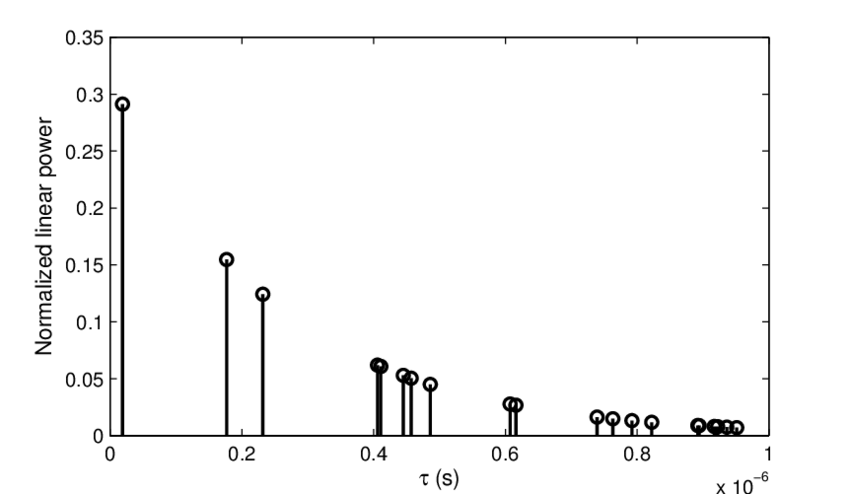
\includegraphics[width=1\linewidth]{figures/delay_spread}
	\caption{Delay Spread}
	\label{fig:delayspread}
\end{figure}

\newpage
\section{Graphical implementation}
before simulating the system we need first to be more familiar with multi-path system we will plot the multi path system we created Figure[\ref{fig:siso-multipath}].


\begin{figure}[!h]
	\centering
	\includegraphics[width=0.7\linewidth]{"figures/SISO Multipath"}
	\caption{}
	\label{fig:siso-multipath}
\end{figure}

\section{Data Generation}
in multi-path we will use a different approach of generating the data.
we will use $10^3$ frames and $10^4$ random bits for each frame.

\subsection{Simulating the system}
in this stage, we are re-simulating the system for each frame and calculating the average BER for each Eb/No.


\newpage
\section{Plotting}
after simulating the system and getting all the values needed, we are ploting the relationship between the BER and Bb/No for SISO multi-path and LOS systems to see the difference between them, and as we can see in Figure[\ref{3245}]

in multi-path graph, it's clear that it does have a higher BER than LOS one.
\begin{figure}[!h]
	\centering
	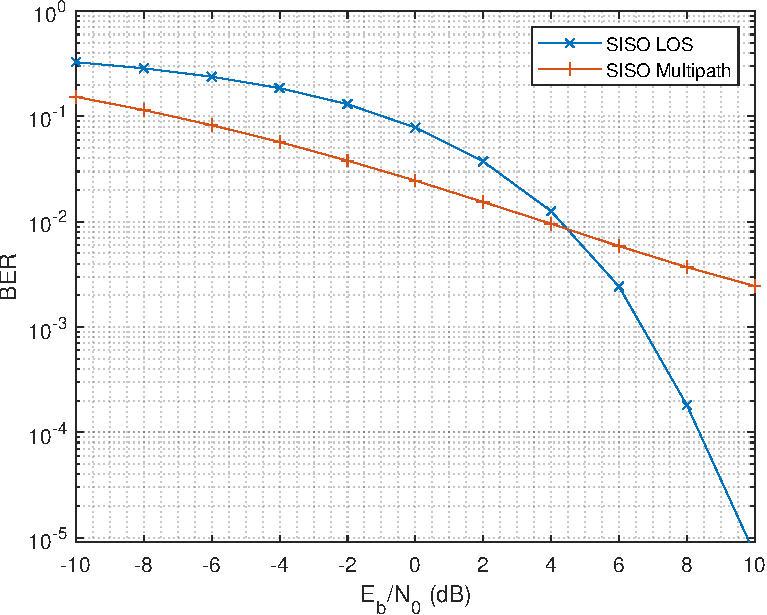
\includegraphics[width=1\linewidth]{figures/SISO_LOS_Multipath.pdf}
	\caption{SISO LOC vs Multi-path}
	\label{3245}
\end{figure}



\newgeometry{margin=0pt}
\newpage
\vfill
\begin{figure}
	\centering
	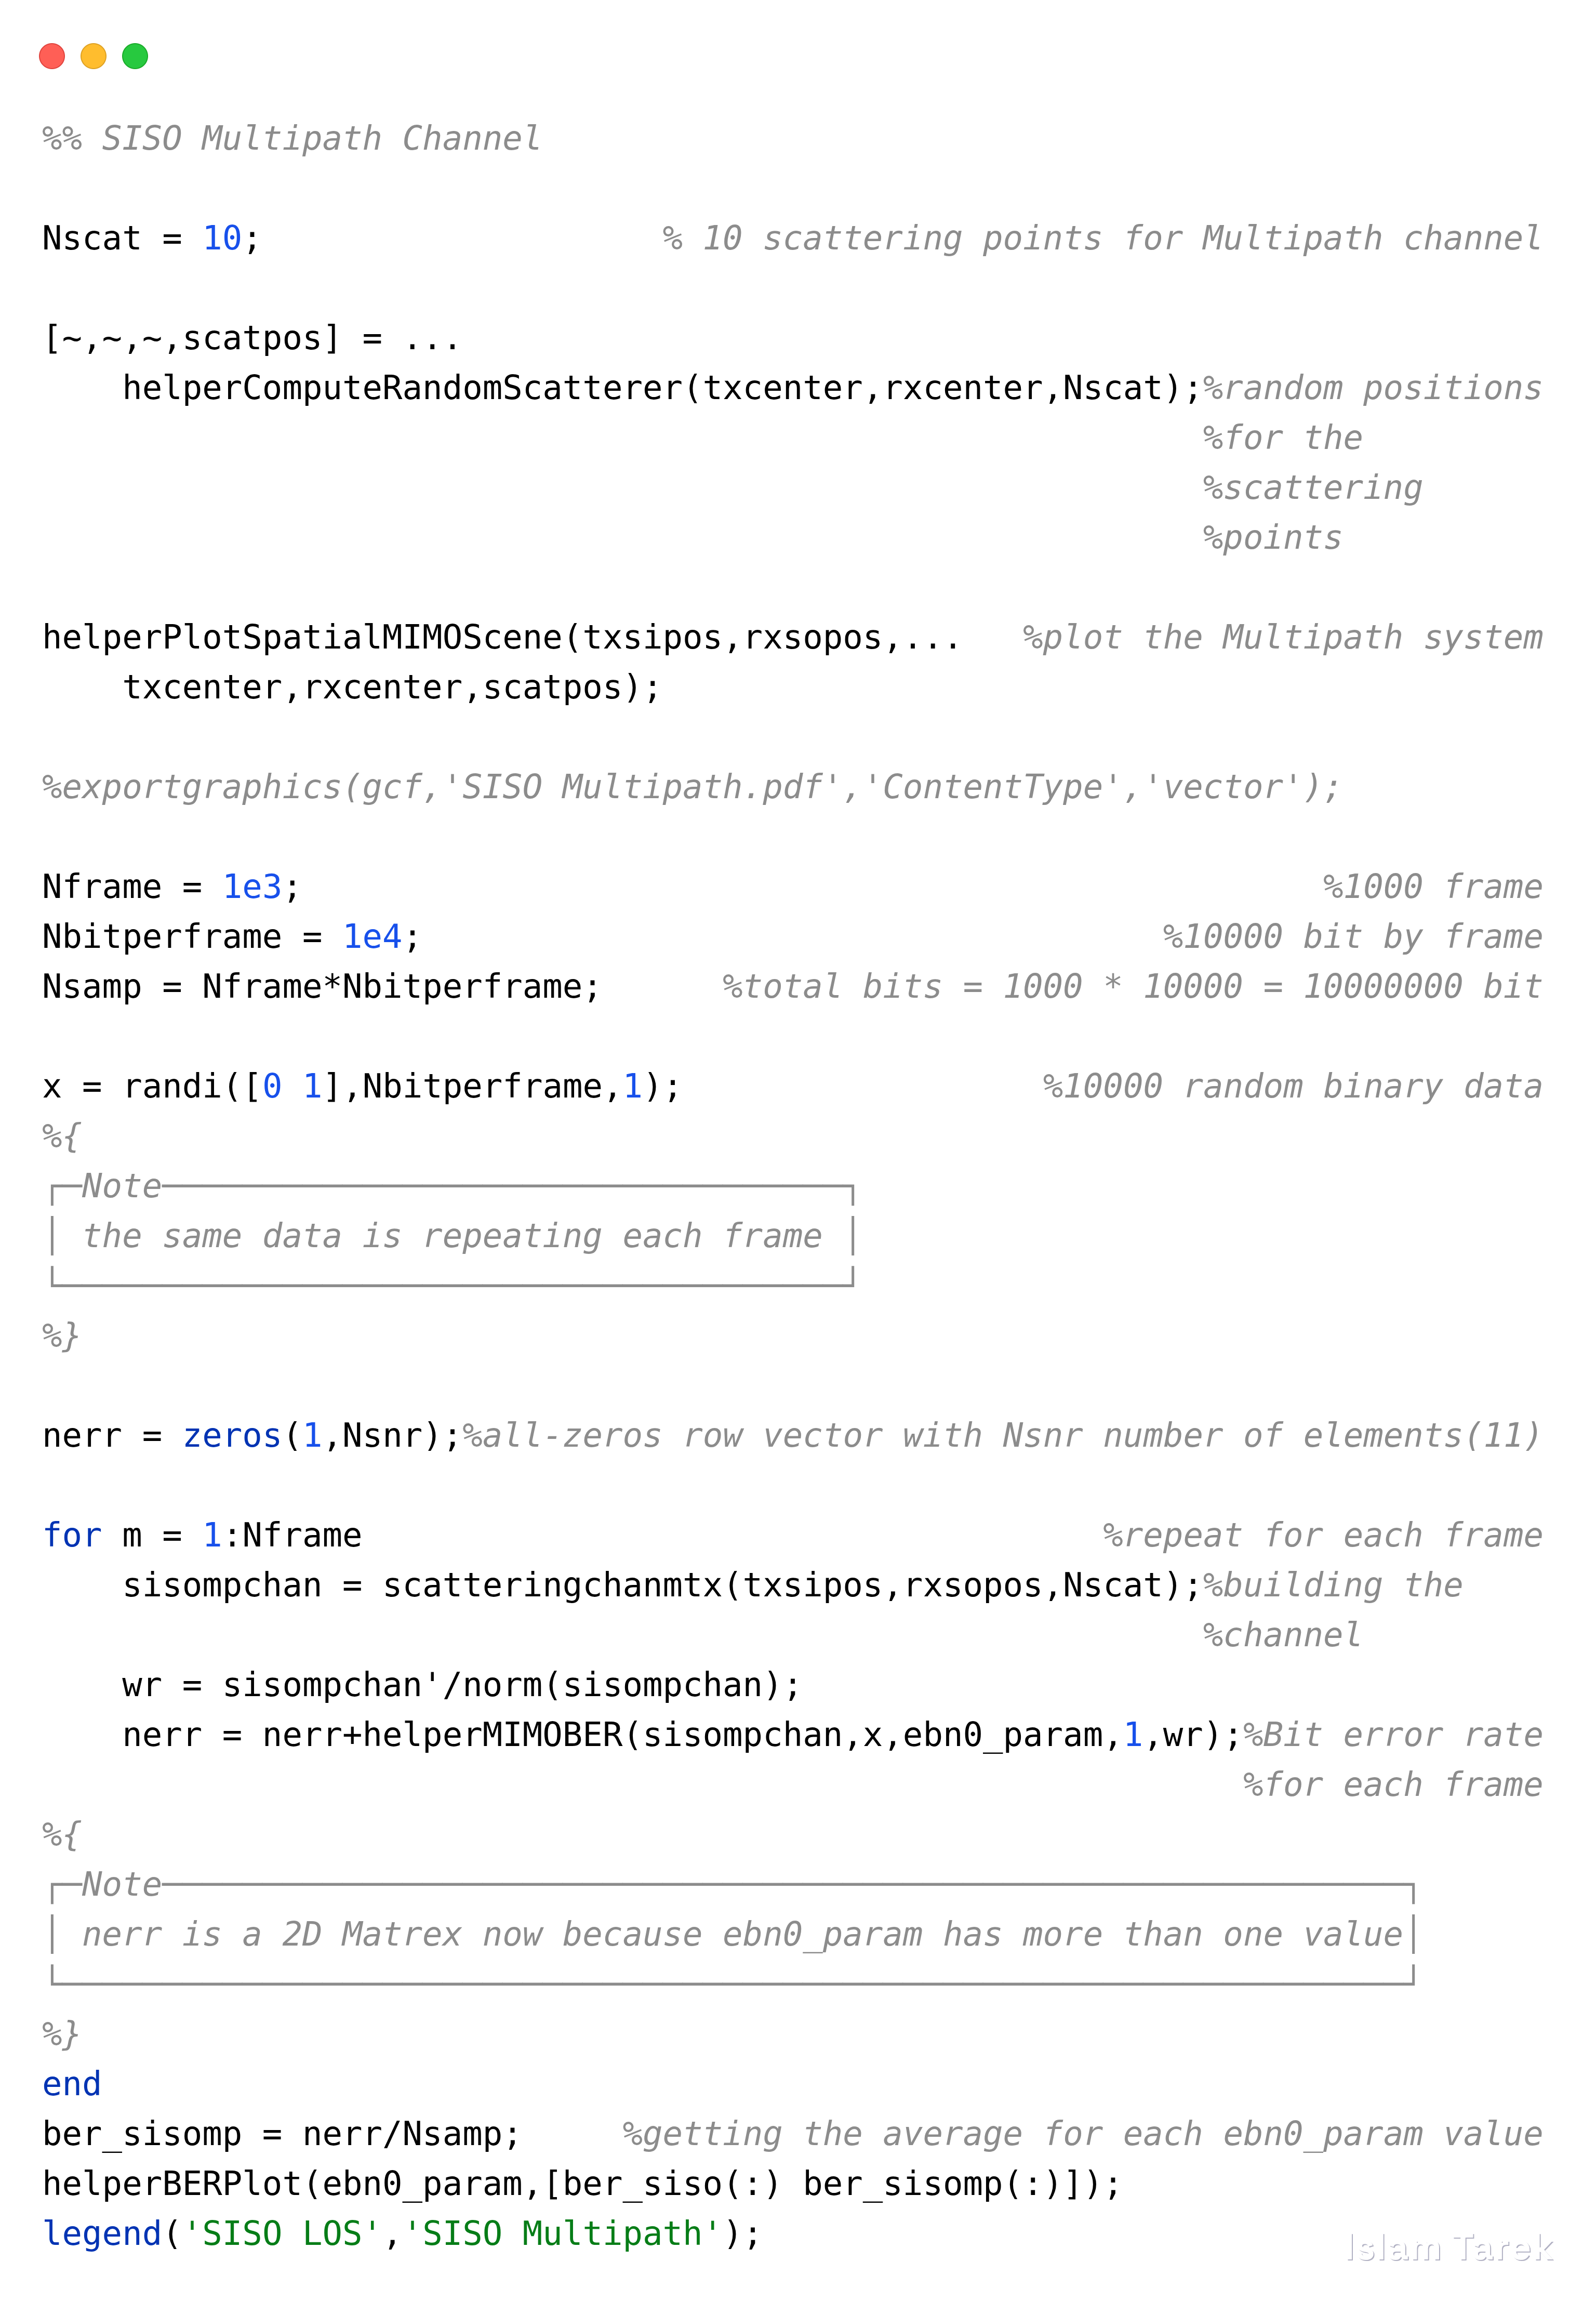
\includegraphics[width=0.7\linewidth]{figures/code6}
\end{figure}
\vfill
\restoregeometry